%%%%%%%%%%%%%%%%%%%%%%%%%%%%%%%%%%%%%%%%%%  不使用 authblk 包制作标题  %%%%%%%%%%%%%%%%%%%%%%%%%%%%%%%%%%%%%%%%%%%%%%
%-------------------------------PPT Title-------------------------------------
\title{05-赝势理论}
%-----------------------------------------------------------------------------

%----------------------------Author & Date------------------------------------
%\author[\textrm{Jun\_Jiang}]{姜\;\;骏\inst{}} %[]{} (optional, use only with lots of authors)
%% - Give the names in the same order as the appear in the paper.
%% - Use the \inst{?} command only if the authors have different
%%   affiliation.
%\institute[BCC]{\inst{}%
\institute[Gain~Strong]{\inst{}%
%\vskip -20pt 北京市计算中心}
\vskip -20pt {\large 格致斯创~科技}}
\date[\today] % (optional, should be abbreviation of conference name)
{%	{\fontsize{6.2pt}{4.2pt}\selectfont{\textcolor{blue}{E-mail:~}\url{jiangjun@bcc.ac.cn}}}
\vskip 45 pt {\fontsize{8.2pt}{6.2pt}\selectfont{%清华大学\;\;物理系% 报告地点
	\vskip 5 pt \textrm{2023.01.07}}}
}

%% - Either use conference name or its abbreviation
%% - Not really information to the audience, more for people (including
%%   yourself) who are reading the slides onlin%%   yourself) who are reading the slides onlin%%   yourself) who are reading the slides onlineee
%%%%%%%%%%%%%%%%%%%%%%%%%%%%%%%%%%%%%%%%%%%%%%%%%%%%%%%%%%%%%%%%%%%%%%%%%%%%%%%%%%%%%%%%%%%%%%%%%%%%%%%%%%%%%%%%%%%%%

\subject{}
% This is only inserted into the PDF information catalog. Can be left
% out.
%\maketitle
\frame
{
%	\frametitle{\fontsize{9.5pt}{5.2pt}\selectfont{\textcolor{orange}{“高通量并发式材料计算算法与软件”年度检查}}}
\titlepage
}
%-----------------------------------------------------------------------------

%------------------------------------------------------------------------------列出全文 outline ---------------------------------------------------------------------------------
%\section*{}
%\frame[allowframebreaks]
%{
%  \frametitle{Outline}
%%  \frametitle{\textcolor{mycolor}{\secname}}
%  \tableofcontents%[current,currentsection,currentsubsection]
%}
%%在每个section之前列出全部Outline
%%类似的在每个subsection之前列出全部Outline是\AtBeginSubsection[]
%\AtBeginSection[]
%{
%  \frame<handout:0>%[allowframebreaks]
%  {
%    \frametitle{Outline}
%%全部Outline中,本部分加亮
%    \tableofcontents[current,currentsection]
%  }
%}

%-----------------------------------------------PPT main Body------------------------------------------------------------------------------------
\small
\frame                               %
{
	\frametitle{\textrm{Kohn-Sham}方程}
\begin{figure}[h!]
\centering
\vspace*{-0.21in}
\hspace*{-0.1in}
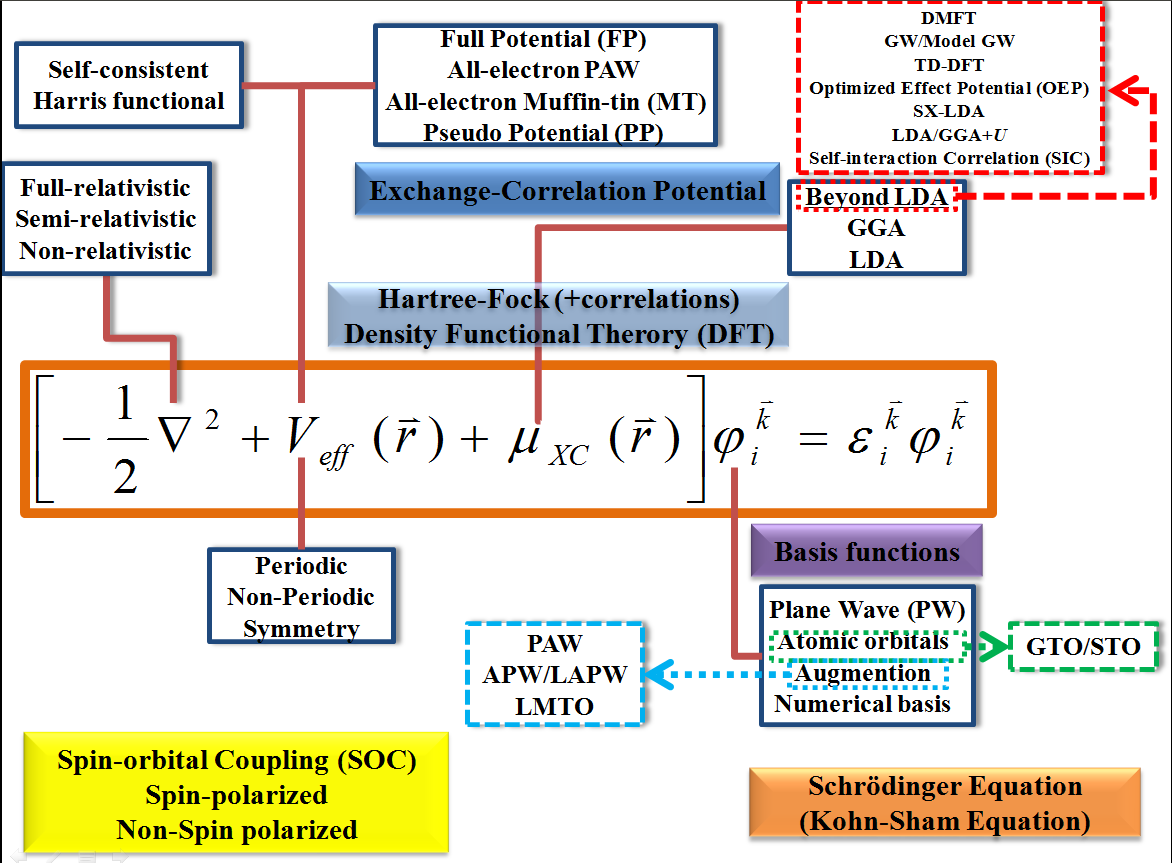
\includegraphics[height=2.7in,width=4.0in,viewport=2 5 1162 880,clip]{Figures/DFT.png}
\caption{\tiny \textrm{The Analysis of Kohn-Sham equation.}}%(与文献\cite{EPJB33-47_2003}图1对比)
\label{DFT}
\end{figure}
}

\section{赝势理论}       %Bookmark
%\section{Induction on DFT and solid-state physics}       %Bookmark
\subsection{平面波与赝势}       %Bookmark
\frame
{
%\frametitle{The methods on band structure calculation}
	\frametitle{由\textrm{OPW~}到赝势}
%\vskip 10pt
%\textrm{The mainly difference of all these methods below: the basis sets and the construction of the potential}
\begin{itemize}
%\setlength{\itemsep}{5pt}
	\item 完全平面波基组\\{\fontsize{7.5pt}{5.5pt}\selectfont{少数平面波就可以很好地描述波函数在原子间的行为,近核波函数则需要大量平面波展开}}%。因此完全平面波基组虽然方便,但求体系本征态对角化的矩阵非常巨大,计算变得异常耗时。
	\item 正交平面波(\textrm{Orthogonalized plane wave, OPW})方法\\{\fontsize{7.5pt}{5.5pt}\selectfont{价电子用与芯层波函数正交的平面波展开
		\begin{displaymath}
			\phi_{\textrm{OPW}}^{\vec k+\vec G}(\vec r)=\phi_{\textrm{PW}}^{\vec k+\vec G}(\vec r)-\sum_c\langle\varphi_c|\phi_{\textrm{PW}}^{\vec k+\vec G}\rangle\varphi_c(\vec r)
		\end{displaymath}}}
	{\fontsize{7.5pt}{5.5pt}\selectfont{构造赝波函数
		\begin{displaymath}
			\tilde{\phi}_v(\vec r)=\phi_v(\vec r)+\sum_c\langle\varphi_c|\tilde{\phi}_v\rangle\varphi_c(\vec r)
		\end{displaymath}
	代入\textrm{Schr\"odinger}方程
		$$\hat H|\tilde{\phi}_v\rangle-\sum_c\langle\varphi_c|\tilde{\phi}_v\rangle\hat H|\varphi_c\rangle=\varepsilon_v|\tilde{\phi}_v\rangle-\varepsilon_v\sum_c\langle\varphi_c|\tilde{\phi}_v\rangle|\varphi_c\rangle$$
		可有$$\hat H|\tilde{\phi}_v\rangle+\textcolor{blue}{V^R}|\tilde{\phi}_v\rangle=\textcolor{blue}{\varepsilon_v}|\tilde{\phi}_v\rangle$$
		这里排斥势是$$V^R(\vec r,\vec r^{\prime})=\sum_c(\varepsilon_v-\varepsilon_c)|\varphi_c(\vec r^{\prime})\rangle\langle\varphi_c(\vec r)|$$}}
\end{itemize}
}

\frame
{
	\frametitle{由\textrm{OPW~}到赝势}
	\textrm{Phillips-Kleinman}指出,赝势($V^{e\!f\!f}$)-赝波函数(可用$\phi_{PW}^{\vec k+\vec G}$展开)满足\textrm{Schr\"odinger}方程%\upcite{PR116-287_1959}
	$$\bigg(-\dfrac12\nabla^2+\textcolor{red}{V^{e\!f\!f}}\bigg)|\tilde{\phi}_v\rangle=\textcolor{blue}{\varepsilon_v}|\tilde{\phi}_v\rangle$$
	其中$\textcolor{red}{V^{e\!f\!f}}=V(\vec r)+\textcolor{blue}{V^R}$
	\begin{itemize}
		\item 赝势-赝波函数的本征值$\varepsilon_v$与真实体系的价电子能量本征值等价
		\item 赝势$\textcolor{red}{V^{e\!f\!f}}$比$V(\vec r)$平滑得多,并且$\textcolor{blue}{V^R}$是非局域的排斥势
			\begin{displaymath}
				\begin{aligned}
					\textcolor{blue}{V^R}f(\vec r)=&\sum_c(\varepsilon_v-\varepsilon_c)\varphi_c(\vec r)\int\varphi_c^{\ast}(\vec r^{\prime})f(\vec r^{\prime})\mathrm{d}\vec r^{\prime} \\
					=&\int V^R(\vec r,\vec r^{\prime})f(\vec r^{\prime})\mathrm{d}\vec r^{\prime}
				\end{aligned}
			\end{displaymath}
%			这里$$V^R(\vec r,\vec r^{\prime})=\sum_c(\varepsilon_v-\varepsilon_c)|\varphi_c(\vec r^{\prime})\rangle\langle\varphi_c(\vec r)|$$
	\end{itemize}
}

\frame
{
\frametitle{赝势的评估}
赝势(\textrm{Pseudo Potential, PP})方法是在正交平面波的基础上发展起来的,构造出平缓的势函数代替核的强吸引作用和芯层电子的排斥作用,用平缓的函数取代波函数近核时的震荡。
\begin{itemize}
\setlength{\itemsep}{5pt}
	\item 赝势-平面波方法,只需要少量平面波可展开赝波函数,大大提升了计算效率;但是赝波函数不能很好地反映与电子近核行为有关的性质。
	\item 赝势的构造并不唯一,考核构造赝势的两大指标:~\\“柔软程度”\textrm{(Soft)}与“可移植性”\textrm{(transferability)}
\end{itemize}
\begin{figure}[h!]
\centering
\vspace*{-0.10in}
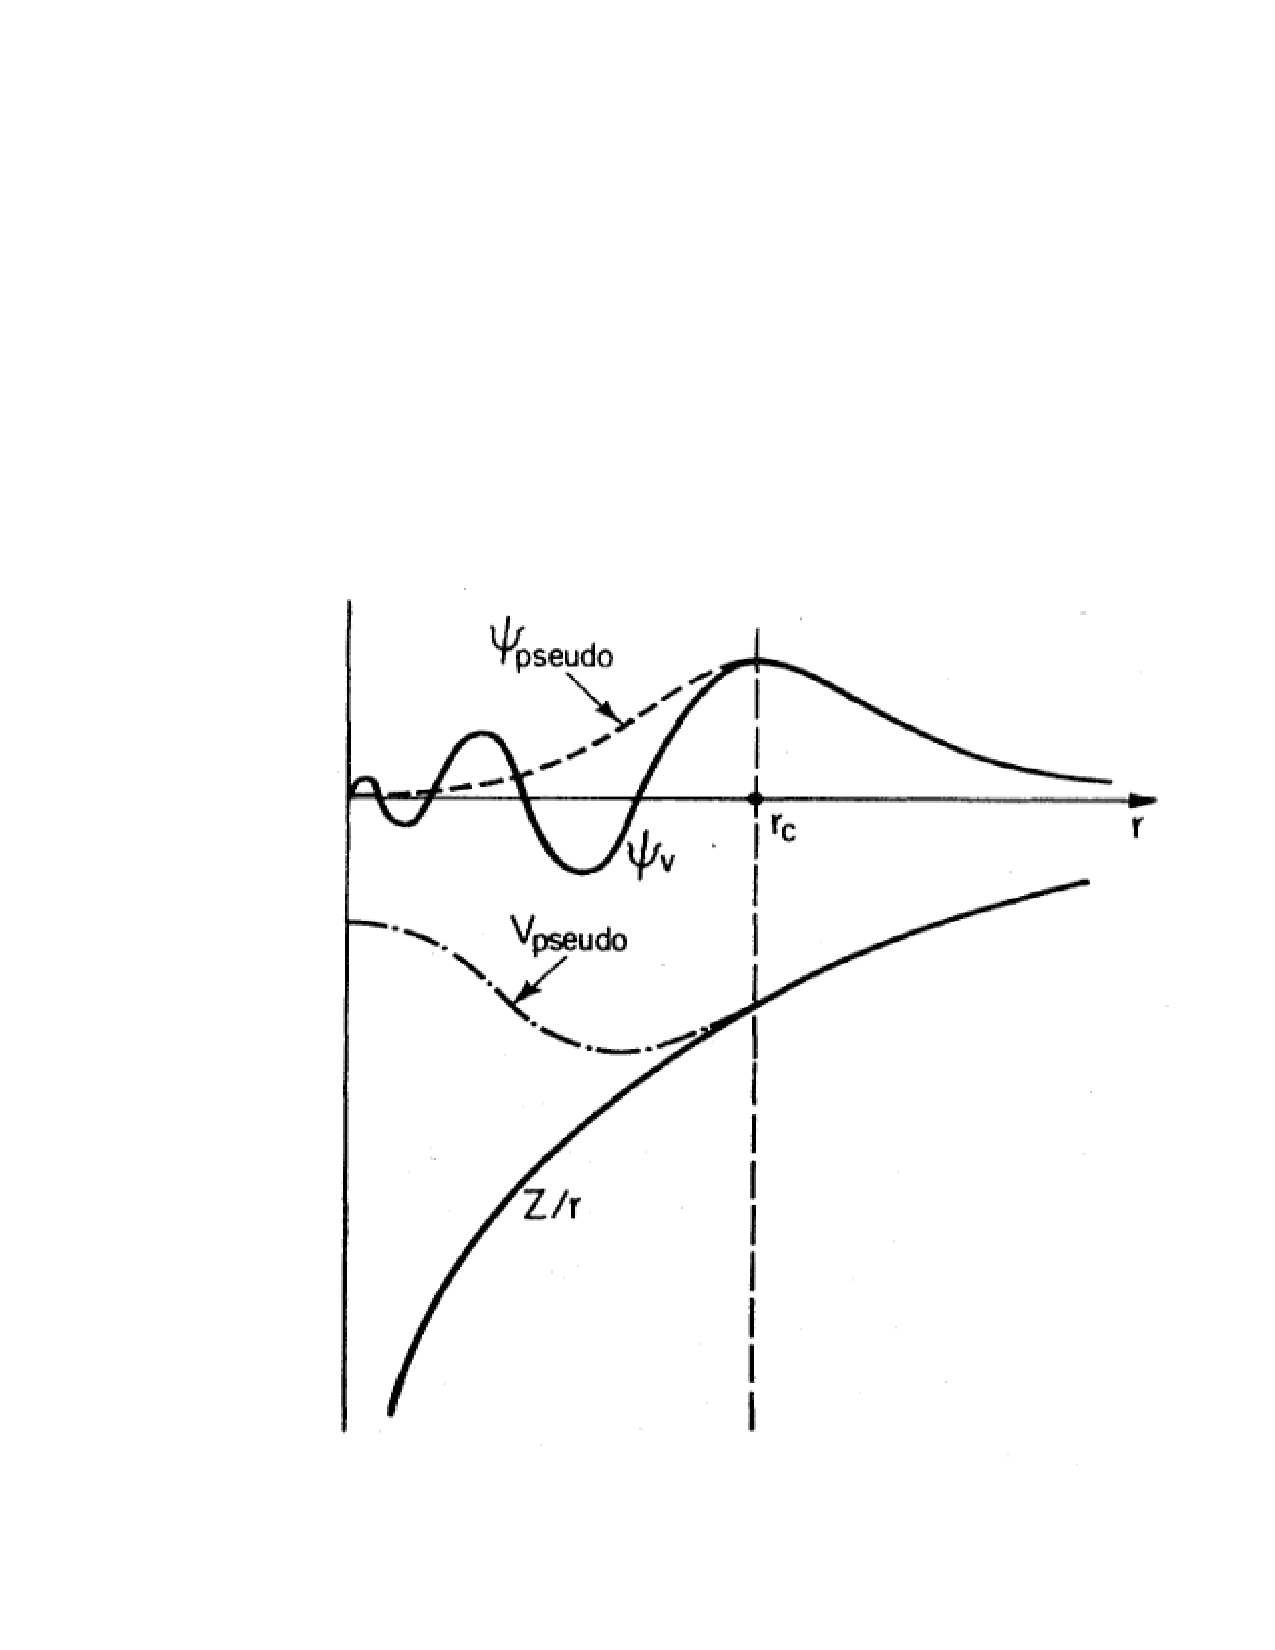
\includegraphics[height=1.35in,width=1.40in,viewport=154 100 562 508,clip]{Figures/Pseudo.pdf}
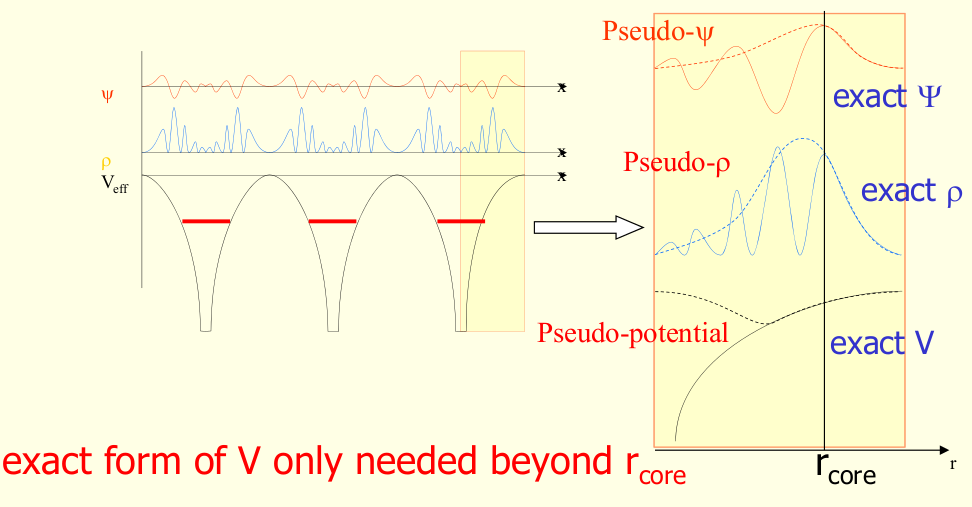
\includegraphics[height=1.35in,width=2.55in,viewport=1 1 980 500,clip]{Figures/Pseudo-2.png}
\caption{\tiny \textrm{The Pseudo wave function and Pseudo potential.}}%(与文献\cite{EPJB33-47_2003}图1对比)
\label{Pseudo_Potential-Wave}
\end{figure}
}

\frame
{
	\frametitle{传统赝势的构造}
	直接由实验数据来确定(模型)赝势,常用的实验数据包括离子对电子的散射角度、离子的光谱实验数据等
		\begin{itemize}
			\item 构造离子赝势:~可移植性好
			\item 构造总赝势(包括全部价电子相互作用):~常用于能带描述
		\end{itemize}
%	\begin{itemize}
%		\item 在指定能量范围内,离子对电子散射的散射角
%		\item 离子的光谱实验数据
%	\end{itemize}
\begin{figure}[h!]
\centering
\vspace*{-0.10in}
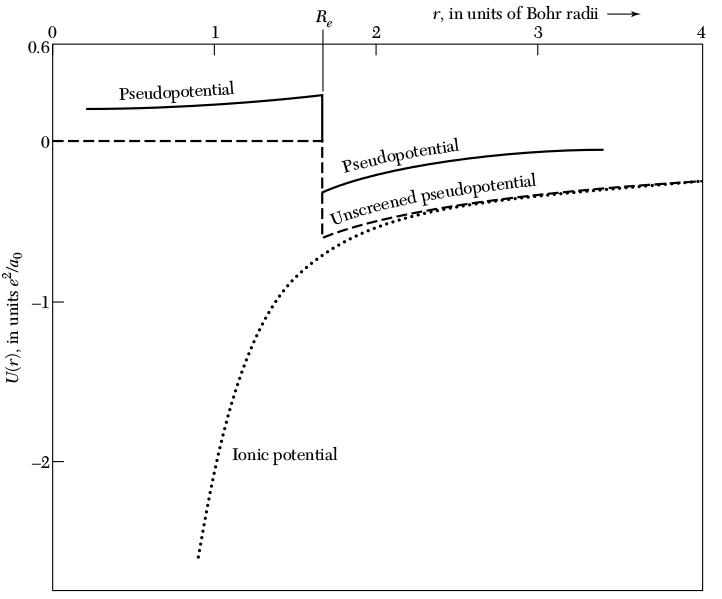
\includegraphics[height=1.60in,width=2.57in,viewport=0 0 980 600,clip]{Figures/Pseudo-model-empty_core.png}
\caption{\tiny \textrm{Pseudopotential for metallic sodium, based on the empty core model and screened by the Thomas-Fermi dielectric function.}}%(与文献\cite{EPJB33-47_2003}图1对比)
\label{Pseudo_model-empty_core}
\end{figure}
}

\frame
{
	\frametitle{传统赝势的构造}
\begin{figure}[h!]
\centering
\vspace*{-0.10in}
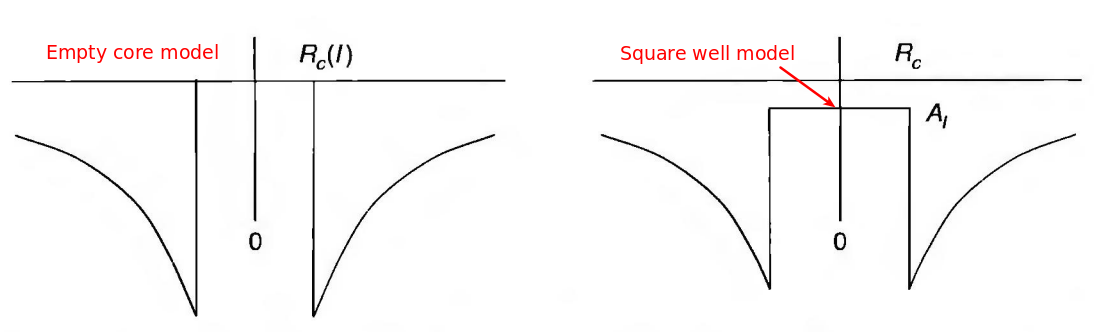
\includegraphics[height=1.30in,width=4.17in,viewport=0 0 1150 350,clip]{Figures/Pseudo-model.png}
\caption{\tiny \textrm{Left:``Empty core'' model potential of Ashcroft in which the potential is zero inside radius $R_c(l)$ which is different for each $l$. Right: Square well model potential with value $A_l$ inside a cut-off radius $R_c$, proposed by Abarenkov and Heine and fit to atomic data by Animalu and Heine. The fact that the potential are weak, zero, or even positive inside cut-off radius $R_c$ is an illustration of the ``cancellation theorem''.}}%(与文献\cite{EPJB33-47_2003}图1对比)
\label{Pseudo-model}
\end{figure}
}

\subsection{模守恒赝势}
\frame
{
	\frametitle{第一原理赝势}
		由第一原理求解出全电子波函数(径向部分)$P_{n,l}(r)$
			\begin{displaymath}
				\bigg[-\dfrac12\dfrac{\mathrm{d}^2}{\mathrm{d}r^2}+\dfrac{l(l+1)}{2r^2}+V(\rho,r)\bigg]P_{n,l}(r)=\varepsilon_{n,l}P_{n,l}(r)
			\end{displaymath}
			这里$V(\rho,r)$是自洽单电子势
			$$V(\rho,r)=-\frac{Z}r+V_{\mathrm H}(\rho,r)+V_{XC}^{\mathrm{LDA}}(\rho(r))$$
			$V_{\mathrm H}(\rho,r)$是\textrm{Hartree}势,$V_{XC}^{\mathrm{LDA}}(\rho(r))$是交换-相关势

			由此构造赝波函数$P_l^{\mathrm{PP}}(r)$,满足
			$$P_l^{\mathrm{PP}}(r)=P_l^{\mathrm{AE}}(r),\quad r>r_{l}^c$$
			进而构造赝势$V_{\mathrm{src},l}^{\mathrm{PP}}(r)$
			$$V_{\mathrm{src},l}^{\mathrm{PP}}(r)=\varepsilon_l-\dfrac{l(l+2)}{2r^2}+\dfrac{1}{2P_l^{\mathrm{PP}}(r)}\dfrac{\mathrm{d}^2}{\mathrm{d}r^2}P_l^{\mathrm{PP}}(r),\quad r<r_{l}^c$$
}

\frame
{
	\frametitle{模守恒\textrm{(Norm-conserving)}条件}
%	构造赝势确定参数的边界(构造条件)
	\begin{enumerate}
		\item 价电子赝波函数的能量本征值与对应全电子波函数能量本征值相等:~$\varepsilon_l^{\mathrm{PP}}=\varepsilon_l^{\mathrm{AE}}$
		\item 价电子赝波函数与真实电子波函数的径向部分在截断半径$r_{c,l}$外相同:~$\psi_l^{\mathrm{PP}}(r)=\psi_l^{\mathrm{AE}}(r),\quad r>r_{l}^c$
		\item 价电子赝波函数与真实电子波函数的对数导数在截断半径$r_{c,l}$处相等:~$D_l^{\mathrm{PP}}(r)=D_l^{\mathrm{AE}}(r),\quad r\geqslant r_{l}^c$\\
		这里$D_l(\varepsilon,r)=r\frac{\psi_l^{\prime}(\varepsilon,r)}{\psi_l(\varepsilon,r)}=r\dfrac{\mathrm{d}}{\mathrm{d}r}\ln\psi_l(\varepsilon,r)$
		\item 价电子赝波函数与真实电子波函数在截断半径$r_{l}^c$内的积分电荷相等(\textcolor{red}{模守恒条件})
			$$Q_l=\int_0^{r_{l}^c}\mathrm{d}rr^2|\psi_l^{\mathrm{PP}}(r)|^2=\int_0^{r_{l}^c}\mathrm{d}rr^2|\psi_l^{\mathrm{AE}}(r)|^2$$
		\item 价电子赝波函数与真实电子波函数的对数导数一阶能量导数$\mathrm{d}D_l(\varepsilon,r)/\mathrm{d}\varepsilon$在截断半径$r_{l}^c$处及以外相等
	\end{enumerate}
}

\frame
{
	\frametitle{模守恒\textrm{(Norm-conserving)}条件}
\begin{figure}[h!]
\centering
\vspace*{-0.10in}
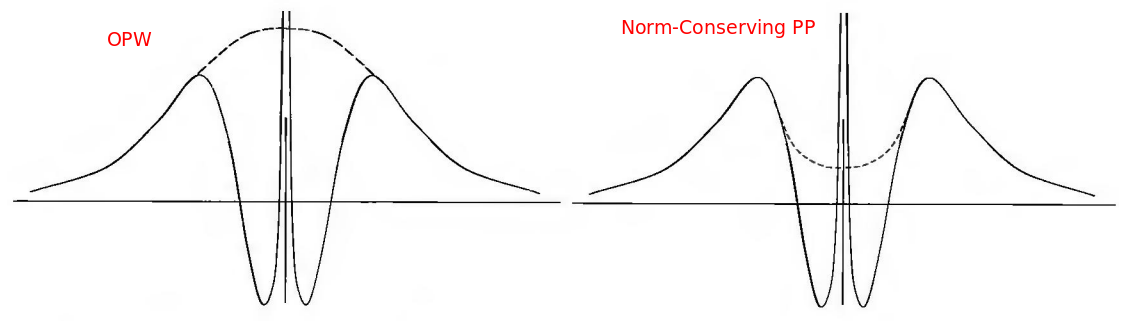
\includegraphics[height=1.30in,width=4.17in,viewport=0 0 1150 350,clip]{Figures/Pseudo-OPW_NCPP.png}
\caption{\tiny \textrm{Schematic example of a valence function that has the character of a $3s$ orbital near the nucleus and two examples of smooth functions (dashed lines) that equal the full wave-function outside the core region. Left: the smooth part of the valence function defined by OPW-like equation; Right: a smooth pseudo-function that satisfies the norm-conservation condition.}}%(与文献\cite{EPJB33-47_2003}图1对比)
\label{Pseudo-OPW_NCPP}
\end{figure}
}

\frame
{
	\frametitle{赝势去屏蔽}
	第一原理赝势建立了赝波函数与对应赝势的一一对应关系,但该赝势包含了电子屏蔽(原子、离子环境)信息,去屏蔽后的赝势对环境依赖更低,“可移植性”更好
	$$V_{\mathrm{ion},l}^{\mathrm{PP}}(r)=V_{\mathrm{src},l}^{\mathrm{PP}}(r)-V_{\mathrm{H},l}^{\mathrm{PP}}(r)-V_{XC,l}^{\mathrm{PP}}(r)$$
	去屏蔽过程中,特别需要注意$V_{XC,l}^{\mathrm{PP}}(r)$的处理
	$$V_{XC,l}^{\mathrm{PP}}(r)=V_{XC}^{\mathrm{PP}}([n_l^{\mathrm{PP}}],r)+\big[V_{XC}^{\mathrm{PP}}([n_l^{\mathrm{PP}}+n^{core}],r)-V_{XC}^{\mathrm{PP}}([n_l^{\mathrm{PP}}],r)\big]$$
}

\frame
{
	\frametitle{非局域赝势}
	当前第一原理赝势径向部分是局域的,但与$l$有关,因此是半局域的(\textrm{semi-local})
	\begin{displaymath}
		\hat{V}^{\mathrm{SL}}=\sum_{lm}|Y_{lm}\rangle V_l(r)\langle Y_{lm}|
	\end{displaymath}
	将赝势的径向部分分解为局域部分($l$无关)和非局域部分($l$相关)
	\begin{displaymath}
		V_{\mathrm{ion},l}^{\mathrm{PP}}(r)=V_{\mathrm{local}}^{\mathrm{PP}}(r)+\delta V_l^{\mathrm{PP}}(r)
	\end{displaymath}
	第一原理赝势可以表示为
	\begin{displaymath}
		\hat{V}^{\mathrm{SL}}=V_{\mathrm{local}}^{\mathrm{PP}}(r)+\sum_{lm}|Y_{lm}\rangle\delta V_l(r)\langle Y_{lm}|
	\end{displaymath}
	赝势的非局域部分可以表示为
	\begin{displaymath}
		\delta V(\vec r,\vec r^{\prime})=\sum_{lm}|Y_{lm}\rangle\delta V_l(r)\langle Y_{lm}|
	\end{displaymath}
}

\subsection{可分离赝势与\rm{Ghost~band}}
\frame
{
	\frametitle{非局域赝势的变量分离}
	\textrm{Kleinman-Bylander}提出了非局域赝势的变量分离的近似方案\footnote{即$\delta V(\vec r,\vec r^{\prime})$可以写成$\delta V(\vec r,\vec r^{\prime})=\sum_{i}f_i(\vec r)g_i(\vec r^{\prime})$的形式}:~\\
%	引入分离算符$\delta V^{\mathrm{NL}}$满足
	{\fontsize{7.2pt}{5.2pt}\selectfont{如果选择适当的局域函数$V_{\mathrm{local}}^{\mathrm{PP}}(r)$,赝势将可分解为局域部分与非局域部分之和:
	$$\hat V_{\mathrm{NL}}^{\mathrm{PP}}(r)=V_{\mathrm{local}}^{\mathrm{PP}}(r)+\sum_{lm}\dfrac{|\psi_{lm}^{\mathrm{PP}}\delta V_l\rangle\langle\delta V_l\psi_{lm}^{\mathrm{PP}}|}{\langle\psi_{lm}^{\mathrm{PP}}|\delta V_l|\psi_{lm}^{\mathrm{PP}}\rangle}$$ 
	\textcolor{magenta}{$\langle\delta V_l(r)\psi_{lm}^{\mathrm{PP}}|$是投影子},这种分解称为\textrm{factored pseudo-potential},方便数值计算
\vskip 10pt
	更一般地,如果允许赝势局域部分$V_{\mathrm{local}}^{\mathrm{PP}}(r)$为任意函数,则可定义辅助函数
	$$\chi_{lm}^{\mathrm{PP}}(\vec r)=\bigg\{\varepsilon_l-\bigg[-\dfrac12\nabla^2+V_{\mathrm{local}}^{\mathrm{PP}}(\vec r)\bigg]\bigg\}\psi_{lm}^{\mathrm{PP}}(\vec r)$$
	于是赝势的非局域部分可表示为
	$$\delta V_{\mathrm{NL}}=\sum_{lm}\dfrac{|\chi_{lm}^{\mathrm{PP}}\rangle\langle\chi_{lm}^{\mathrm{PP}}|}{\langle\chi_{lm}^{\mathrm{PP}}|\psi_{lm}^{\mathrm{PP}}\rangle}$$
$V_{\mathrm{local}}^{\mathrm{PP}}(r)$选择的随意性,将增加计算结果出现\textrm{Ghost~band}的风险
}}
}

\frame
{
	\frametitle{模守恒赝势构造流程}
\begin{figure}[h!]
\centering
%\vspace*{-0.10in}
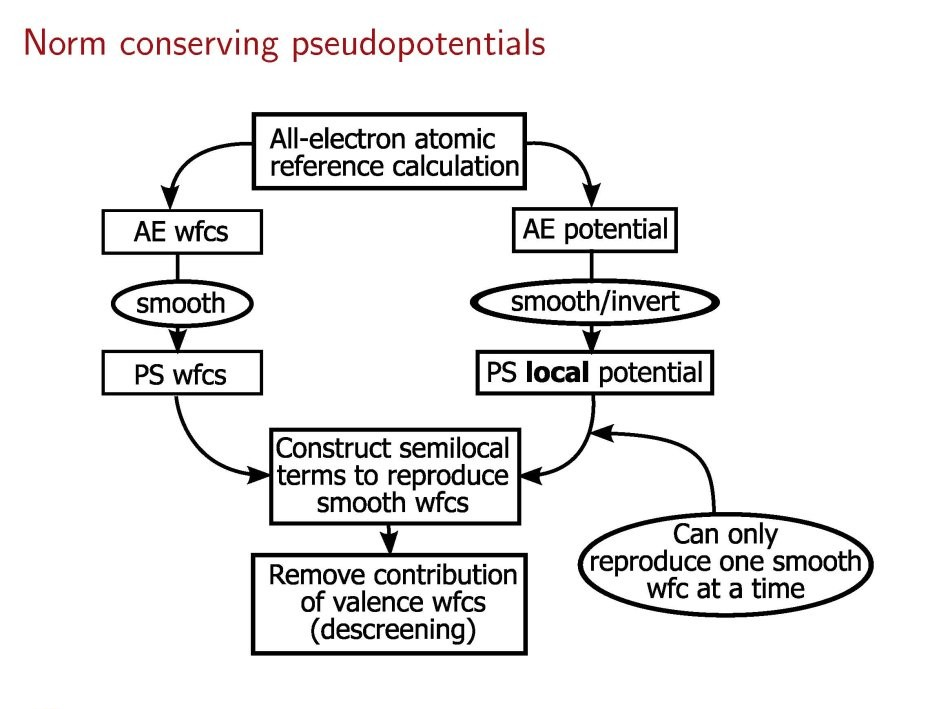
\includegraphics[height=2.70in,width=3.77in,viewport=70 40 900 610,clip]{Figures/Pseudo-NC.jpg}
%\caption{\tiny \textrm{Pseudopotential for metallic sodium, based on the empty core model and screened by the Thomas-Fermi dielectric function.}}%(与文献\cite{EPJB33-47_2003}图1对比)
\label{Pseudo-NC}
\end{figure}
}

\frame
{
	\frametitle{\textrm{Ghost-band}}
	\fontsize{9.2pt}{4.2pt}\selectfont{只有价电子的赝波函数与芯电子波函数完全正交,能带计算中才能确保芯层与价层电子的完全分离。但实际计算时,该正交条件很难严格保证,因此一旦赝波函数严重偏离正交条件,计算的能带中会在本不存在能带的区域出现电子结构分布(称为\textrm{Ghost~band}),这部分电子结构源自构造赝波函数的能量参数$\varepsilon_l$与芯层电子能量差别太大,无法正确描述芯层电荷引起的}
\begin{figure}[h!]
\centering
\vspace*{-0.10in}
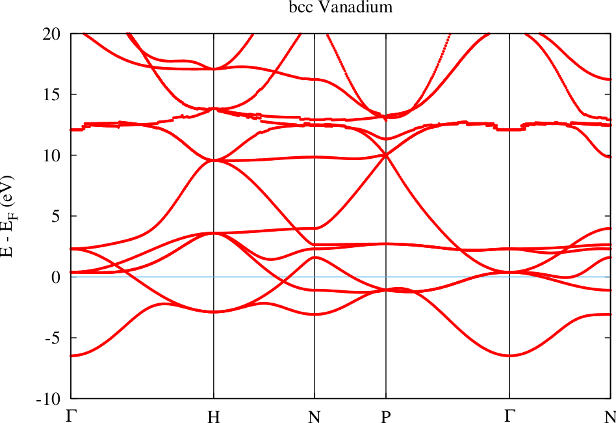
\includegraphics[height=1.50in,width=1.98in,viewport=0 0 450 320,clip]{Figures/Ghostband-Vanadium-1.png}
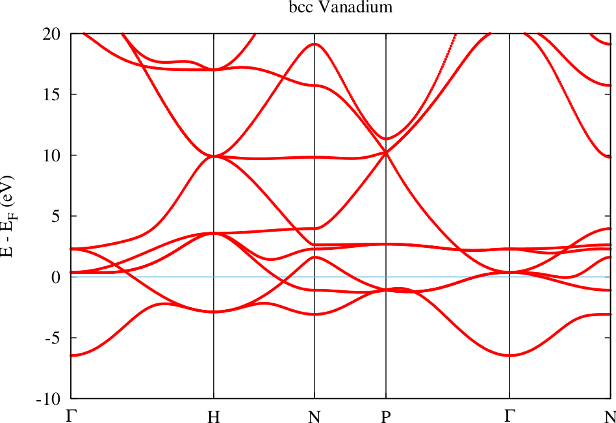
\includegraphics[height=1.50in,width=1.98in,viewport=0 0 450 320,clip]{Figures/Ghostband-Vanadium-4.png}
\caption{\fontsize{7.2pt}{4.2pt}\selectfont{\textrm{The band structure of bcc Vanadium. %In the calculation, all electrons up to the 3p states were treated as core electrons, all other electrons as valence electrons. 
\\Left:~Between 10 and 15 eV above the Fermi energy a strange band with nearly no dispersion can be observed. The vanishing dispersion of the band is a typical property of ghost bands.}}}%(与文献\cite{EPJB33-47_2003}图1对比)
\label{Ghost-band}
\end{figure}
}

\frame
{
	\frametitle{\textrm{Ghost~band}的起源}
	可分离赝势方法中
	\begin{displaymath}
		\hat{\mathbf{H}}=-\dfrac12\nabla^2+V_{\mathrm{local}}(r)+\delta\hat{V}_{\mathrm{NL}}
	\end{displaymath}
	赝波函数$\psi_{lm}^{\mathrm{PP}}(r)$是方程
	\begin{displaymath}
		\hat{\mathbf{H}}\psi_{lm}^{\mathrm{PP}}(r)=\varepsilon_l\psi_{lm}^{\mathrm{PP}}(r)
	\end{displaymath}
	的解。
\vskip 15pt
	因为$V_{\mathrm{local}}(r)$可随意选择,因此赝波函数$\psi_{lm}^{\mathrm{PP}}(r)$和能量$\varepsilon_l$不再要求与束缚态波函数相对应,将导致\textrm{Ghost~band}的出现
}

\frame
{
	\frametitle{\textrm{Ghost~band}的克服}
	{\fontsize{7.2pt}{5.2pt}\selectfont{根据微分方程理论
	\begin{displaymath}
		\hat{\mathbf{H}}\psi_{lm}^{\mathrm{PP}}(r)=\varepsilon_l\psi_{lm}^{\mathrm{PP}}(r)
	\end{displaymath}
	的解$\psi_{lm}^{\mathrm{PP}}(r)$可表示为(只考虑径向部分)
	\begin{displaymath}
		\psi_{l}^{\mathrm{PP}}(r)=u_l^0(r)+\sum_ic_iu_l^i(r)
	\end{displaymath}
这里$u_l^0(r)$和$u_l^i(r)$分别是
齐次微分方程
	\begin{displaymath}
		\bigg(-\dfrac12\nabla^2+V_{\mathrm{local}}-\varepsilon_l^0\bigg)u_{l_0}(r)=0
	\end{displaymath}
和非齐次微分方程
	\begin{displaymath}
		\bigg(-\dfrac12\nabla^2+V_{\mathrm{local}}-\varepsilon_l^j\bigg)u_{l_j}(r)=\chi_{l_j}(r)
	\end{displaymath}
的解

通过引入多个能量参数$\varepsilon_l^i$,优化控制参数$c_i$,可以得到理想的局域势函数$V_{\mathrm{local}}(r)$
}}
}

\frame
{
	\frametitle{广义模守恒条件}
	为提高模守恒赝势的可移植性\footnote{\tiny{换言之,提升赝波函数能适应的能量变分空间}},\textrm{Vanderbilt}和\textrm{Bl\"ochl}分别建议:\\
	在构造可分离赝势时,\textcolor{blue}{引入额外的参考能量$\varepsilon_l$,并要求对每个角动量量子数$l$,所有能量参数$\varepsilon_l$构造的赝波函数$\phi_i^{\mathrm{ps}}$及其辅助函数$\chi_i$都满足
	\begin{displaymath}
		|\chi_i\rangle=-(\mathbf{T}+V_{\mathrm{loc}}-\varepsilon)|\phi_i^{\mathrm{ps}}\rangle
	\end{displaymath}}
	{\fontsize{7.2pt}{5.2pt}\selectfont{这里$i$表示量子数$l$,$m$和能量参数$\varepsilon$,即$i=(lm,\varepsilon)$}}
	\vskip 5pt
	由此出发,可构造出一组与赝波函数$\phi_i^{\mathrm{ps}}$垂直的函数$\beta_i$:~
{\fontsize{7.2pt}{5.2pt}\selectfont{
	\begin{itemize}
		\item 构造矩阵$\mathbf{B}$,其矩阵元$B_{ij}$满足
			\begin{displaymath}
				B_{ij}= \langle\phi_j^{\mathrm{ps}}|\chi_i\rangle
			\end{displaymath}
		\item 由矩阵$\mathbf{B}$和$\chi$得到函数$\beta_i$
			\begin{displaymath}
				|\beta_i\rangle=\sum_j(\mathbf{B}^{-1})_{ij}|\chi_j\rangle
			\end{displaymath}
		\item 由此得到的$\beta$与赝波函数$\phi_i^{\mathrm{ps}}$满足正交条件
	\begin{displaymath}
		\langle\beta_i|\phi_j^{\mathrm{ps}}\rangle=\delta_{ij}
	\end{displaymath}
	\end{itemize}}}
}

\frame
{
	\frametitle{广义模守恒条件}
	因此可分离赝势的非局域部分表示为
	\textcolor{blue}{\begin{displaymath}
		V_{\mathrm{NL}}=\sum_i|\chi_i\rangle\langle\beta_i|=\sum_{ij}B_{ij}|\beta_j\rangle\langle\beta_i|
	\end{displaymath}}
	{\fontsize{7.2pt}{5.2pt}\selectfont{不难看出,如果赝波函数满足广义模守恒条件
	\begin{displaymath}
		Q_{ij}=\langle\phi_j^{\mathrm{AE}}|\phi_i^{\mathrm{AE}}\rangle-\langle\phi_j^{\mathrm{PS}}|\phi_i^{\mathrm{PS}}\rangle = 0
	\end{displaymath}
	亦即
	\begin{displaymath}
		Q_{l\varepsilon,l\varepsilon^{\prime}}=\int_0^{R_c}\bigg(\phi_{l\varepsilon}^{\mathrm{AE}}(r)\phi_{l\epsilon^{\prime}}^{\mathrm{AE}}(r)-\phi_{l\varepsilon}^{\mathrm{PS}}(r)\phi_{l\varepsilon^{\prime}}^{\mathrm{PS}}(r)\bigg)\mathrm{d}r=0
	\end{displaymath}
	将大大提高赝势的可移植性。
	\vskip 5pt
	但实际上,广义模守恒条件看似简单,当能量参数$\varepsilon\neq\varepsilon^{\prime}$,要满足这个条件
	$$Q_{l\varepsilon,l\varepsilon^{\prime}}=0$$
	并非易事;~而一旦模守恒条件被破坏,矩阵$\mathbf{B}$(相应地,赝势的非局域部分$V_{\mathrm{NL}}$)就是非\textrm{Hermitian}}}
}

